\documentclass[10pt]{beamer}
%
%   Arquivo de Configuração dos Slides
%


%
%   Pacotes utilizados
%

% Codificação dos caracteres em formato universal.
\usepackage[utf8]{inputenc}
\usepackage[T1]{fontenc}

% Traduz o texto gerados pelo LaTeX para português. ex.: Capítulo, Seção, Conteúdo.
\usepackage[brazil]{babel}

% Pacotes para ambientes matemáticos
\usepackage{amsmath}
\usepackage{amsthm}
\usepackage{amssymb}

% Diversas funções para o uso das aspas.
\usepackage{csquotes}

% Outros pacotes
\usepackage{hyperref}
\usepackage{tikz}
\usepackage{yfonts}
\usepackage{colortbl}
\usepackage{ragged2e}
\usepackage{helvet}
\usepackage{verbatim}


%
%   Tema
%

% Copyright 2007 by Till Tantau
%
% This file may be distributed and/or modified
%
% 1. under the LaTeX Project Public License and/or
% 2. under the GNU Public License.
%
% See the file doc/licenses/LICENSE for more details.


% Common packages


\usepackage[brazil]{babel}
\usepackage[utf8]{inputenc}
\usepackage{times}
 \mode<article> {
  \usepackage{times}
  \usepackage{mathptmx}
  \usepackage[left=1.5cm,right=6cm,top=1.5cm,bottom=3cm]{geometry}
}

\usepackage{hyperref}
\usepackage[T1]{fontenc}
\usepackage{amsmath,amssymb}
\usepackage{tikz}
\usepackage{colortbl}
\usepackage{yfonts}
\usepackage{colortbl}
\usepackage{translator} % comment this, if not available
\usepackage{ragged2e} % justifying
% Or whatever. Note that the encoding and the font should match. If T1
% does not look nice, try deleting the line with the fontenc.
\usepackage{helvet}
\usepackage{verbatim}


%\usepackage{lipsum}
%\usepackage{enumitem}


\usetheme[
%%% options passed to the outer theme
%    hidetitle,           % hide the (short) title in the sidebar
%    hideauthor,          % hide the (short) author in the sidebar
%    hideinstitute,       % hide the (short) institute in the bottom of the sidebar
%    shownavsym,          % show the navigation symbols
%    width=2cm,           % width of the sidebar (default is 2 cm)
%    hideothersubsections,% hide all subsections but the subsections in the current section
%    hideallsubsections,  % hide all subsections
    right               % right of left position of sidebar (default is right)
%%% options passed to the color theme
%    lightheaderbg,       % use a light header background
  ]{AAUsidebar}

% If you want to change the colors of the various elements in the theme, edit and uncomment the following lines
% Change the bar and sidebar colors:
%\setbeamercolor{AAUsidebar}{fg=red!20,bg=red}
%\setbeamercolor{sidebar}{bg=red!20}
% Change the color of the structural elements:
%\setbeamercolor{structure}{fg=red}
% Change the frame title text color:
%\setbeamercolor{frametitle}{fg=blue}
% Change the normal text color background:
%\setbeamercolor{normal text}{bg=gray!10}
% Highlight the text in the sidebar
\usecolortheme{rose,sidebartab}
% ... and you can of course change a lot more - see the beamer user manual.

% colored hyperlinks
\newcommand{\chref}[2]{%
  \href{#1}{{\usebeamercolor[bg]{AAUsidebar}#2}}%
}


\newcommand{\prn}[1]{\left(#1\right)}

% specify a logo on the titlepage (you can specify additional logos an include them in
% institute command below
\pgfdeclareimage[height=1cm]{titlepagelogo}{theme/figures/ufrn2} % placed on the title page
\pgfdeclareimage[height=1cm]{titlepagelogo2}{theme/figures/imd} % placed on the title page
\titlegraphic{% is placed on the bottom of the title page
  \pgfuseimage{titlepagelogo}
  \hspace{1cm}\pgfuseimage{titlepagelogo2}
}


% Article version layout settings

\mode<article>

\makeatletter
\def\@listI{\leftmargin\leftmargini
  \parsep 0pt
  \topsep 5\p@   \@plus3\p@ \@minus5\p@
  \itemsep0pt}
\let\@listi=\@listI


\setbeamertemplate{frametitle}{\paragraph*{\insertframetitle\
    \ \small\insertframesubtitle}\ \par
}
\setbeamertemplate{frame end}{%
  \marginpar{\scriptsize\hbox to 1cm{\sffamily%
      \hfill\strut\insertshortlecture.\insertframenumber}\hrule height .2pt}}
\setlength{\marginparwidth}{1cm}
\setlength{\marginparsep}{4.5cm}

\def\@maketitle{\makechapter}

\def\makechapter{
  \newpage
  \null
  \vskip 2em%
  {%
    \parindent=0pt
    \raggedright
    \sffamily
    \vskip8pt
    
\includegraphics[width=\linewidth]{theme/figures/imd.png}\par\vskip2em
    {\fontsize{36pt}{36pt}\selectfont Aula \insertshortlecture \par\vskip2pt}
    {\fontsize{24pt}{28pt}\selectfont \color{blue!50!black} \@title\par\vskip4pt}
    %{\Large\selectfont \color{blue!50!black} \insertsubtitle\par}
    \vskip10pt

    \normalsize\selectfont [Notas de Aula]
    Disciplina: \emph{\lecturename \ (\semestre)} \par\vskip1.5em
    \nomedoautor\hskip1em Email: \ \emaildoautor
  }
  \par
  \vskip 1.5em%
}

\let\origstartsection=\@startsection
\def\@startsection#1#2#3#4#5#6{%
  \origstartsection{#1}{#2}{#3}{#4}{#5}{#6\normalfont\sffamily\color{blue!50!black}\selectfont}}

\makeatother

\mode
<all>




% Typesetting Listings

\usepackage{listings}
\lstset{language=Java}

\alt<presentation>
{\lstset{%
  basicstyle=\footnotesize\ttfamily,
  commentstyle=\slshape\color{green!50!black},
  keywordstyle=\bfseries\color{blue!50!black},
  identifierstyle=\color{blue},
  stringstyle=\color{orange},
  escapechar=\#,
  emphstyle=\color{red}}
}
{
  \lstset{%
    basicstyle=\ttfamily,
    keywordstyle=\bfseries,
    commentstyle=\itshape,
    escapechar=\#,
    emphstyle=\bfseries\color{red}
  }
}



% Common theorem-like environments
%\usepackage{amsthm}

\setbeamertemplate{theorems}[numbered]

\theoremstyle{plain}
\newtheorem{Teo}{Teorema}


\theoremstyle{definition}

\newtheorem{Def}[Teo]{Definição}
\newtheorem{exercise}{Exercício}

\theoremstyle{remark}

\newtheorem{Obs}[Teo]{Observação}




\newtheorem{Exer}[Teo]{Exercicio Resolvido}%{\translate{Exercise}}

\newtheorem{Cor}[Teo]{Corolário}
\newtheorem{Exem}[Teo]{Exemplo}
\newtheorem{Lem}[Teo]{Lema}
\newtheorem{Prop}[Teo]{Proposição}
\newtheorem{Sumario}[Teo]{Sumário}
\newtheorem{Obse}{Observação}

\newcounter{Listaexercicios}
\def\Ex#1{
\stepcounter{Listaexercicios} \textbf{\arabic{Listaexercicios}}. #1
}




% New useful definitions:

\newbox\mytempbox
\newdimen\mytempdimen

\newcommand\includegraphicscopyright[3][]{%
  \leavevmode\vbox{\vskip3pt\raggedright\setbox\mytempbox=\hbox{\includegraphics[#1]{#2}}%
    \mytempdimen=\wd\mytempbox\box\mytempbox\par\vskip1pt%
    \fontsize{3}{3.5}\selectfont{\color{black!25}{\vbox{\hsize=\mytempdimen#3}}}\vskip3pt%
}}

\newenvironment{colortabular}[1]{\medskip\rowcolors[]{1}{blue!20}{blue!10}\tabular{#1}\rowcolor{blue!40}}{\endtabular\medskip}

\def\equad{\leavevmode\hbox{}\quad}

\newenvironment{greencolortabular}[1]
{\medskip\rowcolors[]{1}{green!50!black!20}{green!50!black!10}%
  \tabular{#1}\rowcolor{green!50!black!40}}%
{\endtabular\medskip}

%\setbeamertemplate{theorem begin}{{ \inserttheoremheadfont
%\inserttheoremname \inserttheoremnumber
%\ifx\inserttheoremaddition\empty\else\ (\inserttheoremaddition)\fi%
%\inserttheorempunctuation }} \setbeamertemplate{theorem end}{}

\newcommand{\vu}{\vec{u}}
\newcommand{\vv}{\vec{v}}
\newcommand{\vi}{\vec{i}}
\newcommand{\vj}{\vec{j}}
\newcommand{\vk}{\vec{k}}
\newcommand{\vw}{\vec{w}}
\newcommand{\R}{\mathbb{R}}
\newcommand{\N}{\mathbb{N}}
\newcommand{\Z}{\mathbb{Z}}
\newcommand{\Q}{\mathbb{Q}}
\newcommand{\C}{\mathbb{C}}
\newcommand{\U}{\mathcal U}
\newcommand{\I}{\mathcal I}
\newcommand{\sen}{\text{sen}}
\newcommand\seg[2]{\overline{#1#2}}
\def\set#1{\left\{#1\right\}}
\def\paren#1{\left(#1\right)}
\def\colc#1{\left[#1\right]}
\def\modu#1{\left|#1\right|}
\def\tq{\;;\;}
\def\sub#1{\underline{#1}}
\def\link#1#2{\href{#1}{{\tt #2}}}



%
%   Macros
%

\usepackage{macros/macros}


%
%   Ambientes
%

\theoremstyle{plain}
\newtheorem{teorema}{Teorema}

\theoremstyle{definition}
\newtheorem{definicao}[teorema]{Definição}
%\newtheorem{exercicio}{Exercício}

\theoremstyle{remark}
\newtheorem{obs}[teorema]{Observação}
\newtheorem{observacao}[teorema]{Observação}
\newtheorem{corolario}[teorema]{Corolário}
\newtheorem{exemplo}[teorema]{Exemplo}
\newtheorem{lema}[teorema]{Lema}
\newtheorem{proposicao}[teorema]{Proposição}

\newcounter{exercicios}
\newenvironment{exercicio}{\stepcounter{exercicios} \textbf{\arabic{exercicios}}.}{}

% compatibilidade
\newcommand{\Ex}[1]{\begin{exercicio}#1\end{exercicio}}

%
%   Definições e comandos auxiliares do preâmbulo
%

\newcommand{\capitulo}[1]{\lecture[#1]{Capítulo}}
\newcommand{\aula}[1]{\subtitle{#1}}
\newcommand{\autor}{Igor Oliveira}
\newcommand{\email}{\href{mailto:matematicaelementar@imd.ufrn.br}{\texttt{matematicaelementar@imd.ufrn.br}}}
\newcommand{\disciplina}{Matemática Elementar}
\newcommand{\codigo}{IMD1001}

\title{\disciplina}
\date{\today}
\author[\autor]
{
    \autor\\
    \email
}

\def\lecturename{\codigo

\disciplina}

\institute[
	UFRN\\
	Natal-RN
]
{
	Instituto Metrópole Digital\\
	Universidade Federal do Rio Grande do Norte\\
	Natal-RN

}

% compatibilidade
\newcommand{\vu}{\vec{u}}
\newcommand{\vv}{\vec{v}}
\newcommand{\vi}{\vec{i}}
\newcommand{\vj}{\vec{j}}
\newcommand{\vk}{\vec{k}}
\newcommand{\vw}{\vec{w}}
\newcommand{\segmento}[2]{\overline{#1#2}}
\def\colc#1{\left[#1\right]}
\newcommand{\negacao}{\sim}

\justifying


\aula{Funções Polinomiais}
\capitulo{8}


\begin{document}	

	%
	%	Capa
	%

	{\backgroundimage\begin{frame}[plain]
		\titlepage
	\end{frame}}


	%
	%	Sumário
	%

	\begin{frame}
		\frametitle{Índice}
		\tableofcontents
	\end{frame}


	%
	%	Seções
	%

\section{Introdução}

\begin{frame}  \frametitle{Apresentação da Aula}

É algo  comum escutar a seguinte frase: "Em matemática eu resolvo
tudo com regra de três".

Será mesmo que isso é possível? Por exemplo, o lado do quadrado e
sua área são proporcionais?


\end{frame}

%------------------------------------------------------------------------------------------------------------

\section{Função Linear}
\begin{frame} \frametitle{Função Linear}
\begin{definicao}
Chamamos de \sub{função linear} uma função real com lei de formação
$f(x) = ax$.
\end{definicao}\pause

A função linear é usada para modelar problemas de proporcionalidade
direta. Quando duas grandezas são diretamente proporcionais, podemos
escrevê-las sob a lei de formação de uma função linear.

Note que, sabendo que uma função é linear, o valor de $a$ é igual a
$f(1)$.\pause

No caso das grandezas inversamente proporcionais, a função
matemática que modela tal problema é uma função $f: \R^{\ast} \to
\R^{\ast}$ tal que $f(x) = \frac a x$. Nesse caso, também temos a
particularidade de $f(1) = a \in \R^{\ast}$.



\end{frame}

%------------------------------------------------------------------------------------------------------------

\begin{frame}
\frametitle{Função Linear} %\framesubtitle{Exemplos}

\begin{teorema}[Teorema Fundamental da Proporcionalidade]
Seja $f: \R \to \R$ uma função crescente. As seguintes afirmações
são equivalentes:
\begin{enumerate}[(i)]
	\item  $f$ é linear;
	\item $f(x+y) = f(x) + f(y)$ para quaisquer $x, y \in \R$;
	\item $f(nx) = nf(x)$ para todo $n \in \Z$ e todo $x \in \R$.
\end{enumerate}
\end{teorema}
Nas hipóteses do Teorema, tem-se $a=f(1) > 0$. No caso de se supor
$f$ decrescente, vale um resultado análogo, com $a<0$.

\end{frame}

%------------------------------------------------------------------------------------------------------------

\begin{frame}
\frametitle{Função Linear} %\framesubtitle{Exemplos}

A importância desse Teorema está no seguinte fato: se queremos saber
se $f: \R \to \R$ é uma função linear, basta verificar duas coisas:
\begin{enumerate}[1ª:]
	\item $f$ deve ser crescente ou decrescente. (Estamos deixando de
	lado o caso trivial de $f$ ser identicamente nula);
	\item $f(nx) = n f(x)$ para todo $x \in \R$ e todo $n \in \Z$. No
	caso de $f: \R^+ \to \R^+$, basta verificar essa última condição
	para $n \in \N$.
\end{enumerate}

\end{frame}



%------------------------------------------------------------------------------------------------------------
\begin{frame}
\frametitle{Função Linear} %\framesubtitle{Exemplos}

\begin{exemplo}
O lado de um quadrado é proporcional à sua área? Em outras palavras,
essas duas grandezas podem ser relacionadas por meio de uma função
linear?
\end{exemplo}

\end{frame}



%------------------------------------------------------------------------------------------------------------
\section{Função Afim}
\begin{frame}
\frametitle{Função Afim} %\framesubtitle{Exemplos}

\begin{definicao}
Uma função real chama-se \sub{afim} quando existem constantes $a, b
\in \R$ tais que $f(x) = ax +b$ para todo $x\in \R$.
\end{definicao}

Em uma função afim na qual $f(x) = ax +b$, chamamos o valor $a$ de
\sub{taxa de variação} da função ou de \sub{taxa de crescimento}.\\
Vale observar que é muito comum chamá-lo de coeficiente angular.
Esse termo não é apropriado pois define-se coeficiente angular para
retas, e não para funções, mesmo que vejamos que o gráfico de uma
função afim seja uma reta.

\end{frame}


%------------------------------------------------------------------------------------------------------------
\begin{frame}
\frametitle{Função Afim} %\framesubtitle{Exemplos}

\begin{exemplo}
A função identidade $f: \R \to \R$, definida por $f(x) = x$ para
todo $x \in \R$, é afim, assim como suas translações $g(x) = x+b$.
São, ainda, casos particulares de funções afins as funções lineares
$f(x) = ax$ e as funções constantes $f(x) = b$.
\end{exemplo}\pause

\begin{exemplo}
O preço a se pagar por uma corrida de táxi é dado por uma função
afim $f: x \mapsto ax+b$, em que $x$ é a distância percorrida
(usualmente medida em quilômetros), o valor inicial $b$ é a chamada
\emph{bandeirada} e o coeficiente $a$ é o preço de cada quilômetro
rodado.
\end{exemplo}

\end{frame}


%------------------------------------------------------------------------------------------------------------
\begin{frame}
\frametitle{Gráfico da Função Afim} %\framesubtitle{Exemplos}
\begin{proposicao}
O gráfico de uma função afim $f(x) = ax + b$ é uma reta.
\end{proposicao}\pause
Note que, para desenhar o gráfico de uma função afim, basta conhecer
dois pontos, pois uma reta é inteiramente determinada por dois
pontos.

\end{frame}


%------------------------------------------------------------------------------------------------------------
\begin{frame}
\frametitle{Função Afim e PA} %\framesubtitle{Exemplos}

\begin{proposicao}
Seja  $f: \R \to \R$. Se $f$ é uma função afim e $\paren{x_1, x_2,
\dots , x_i, \dots}$ é uma PA, então a sequência formada pelos
pontos $y_i = f(x_i)$, $i \in \N^{\ast}$ é uma PA. Reciprocamente,
se $f$ for monótona e transformar qualquer PA $\paren{x_1, x_2,
\dots , x_i, \dots}$ numa PA com termo geral $y_i = f(x_i)$, $i \in
\N^{\ast}$, então $f$ é uma função afim.
\end{proposicao}


\end{frame}

%------------------------------------------------------------------------------------------------------------

\section{Atividade Online}
\begin{frame}
\frametitle{Atividade Online} %\framesubtitle{Exemplos}

OBSERVAÇÃO: No Khan Academy é definido função linear como função
afim. Ou seja, para eles é qualquer função que o gráfico é uma reta
(ou pontos colineares).

\href{https://pt.khanacademy.org/math/cc-eighth-grade-math/cc-8th-linear-equations-functions/8th-linear-functions-modeling/e/constructing-and-interpreting-linear-functions}
{{\tt Atividade 01 - Problemas de Modelos de Funções Lineares}}

\href{https://pt.khanacademy.org/math/cc-eighth-grade-math/cc-8th-linear-equations-functions/constructing-linear-models-real-world/e/constructing-linear-functions-word-problems}
{{\tt Atividade 02 - Problemas de Como Escrever Funções}}

\href{https://pt.khanacademy.org/math/cc-eighth-grade-math/cc-8th-linear-equations-functions/linear-nonlinear-functions-tut/e/linear-non-linear-functions}
{{\tt Atividade 03 - Funções Lineares e Não Lineares}}

Veja o desempenho na Missão 9º ano.


\end{frame}

%------------------------------------------------------------------------------------------------------------
\section{Função Quadrática}
\begin{frame}
\frametitle{Função Quadrática} %\framesubtitle{Exemplos}

\begin{definicao}
Uma função $f: \R \to \R$ chama-se \sub{quadrática} quando existem
números reais $a, b, c$, com $a \neq 0$, tais que $f(x) = ax^2 +bx
+c$ para todo $x \in \R$.
\end{definicao}


\end{frame}

%------------------------------------------------------------------------------------------------------------

\begin{frame}
\frametitle{Função Quadrática} %\framesubtitle{Exemplos}

\begin{proposicao}
Seja $f$ uma função quadrática da forma $f(x) = ax^2 + bx +c$, onde
$a >0$.\\
Mostre que $f$ não é limitada superiormente e que o ponto
$\paren{-\frac {b} {2a}, -\frac {\Delta} {4a}}$ é o mínimo absoluto
da função.\\
Caso tenhamos $a<0$, então $f$ não é limitada inferiormente e  o
ponto $\paren{-\frac {b} {2a}, -\frac {\Delta} {4a}}$ é o máximo
absoluto da função.
\end{proposicao}\pause

\begin{proposicao}
Seja $f$ uma função quadrática da forma $f(x) = ax^2 + bx +c$. Se
$f(x_1) = f(x_2)$ para $x_1 \neq x_2$, então $x_1$ e $x_2$ são
equidistantes de $-\frac{b} {2a}$, ou seja, $\frac{x_1 +x_2} 2 =
-\frac{b}{2a}$.
\end{proposicao}

\end{frame}

%------------------------------------------------------------------------------------------------------------

\begin{frame}
\frametitle{O Gráfico da Função Quadrática} %\framesubtitle{Exemplos}

\begin{exemplo}
O gráfico da função quadrática $f(x) = ax^2$ é uma parábola cujo
foco é $F = \paren{0, \frac 1 {4a}}$ e cuja diretriz é a reta
horizontal $y = -\frac{1}{4a}$. Ademais, o vértice da parábola é a
origem do plano cartesiano.
\end{exemplo}\pause

\begin{proposicao}
O gráfico de uma função quadrática $f(x) = ax^2 + bx + c$ é uma
parábola, tem a reta $x = -\frac {b}{2a}$ como eixo de simetria e o
ponto $\paren{-\frac {b} {2a}, -\frac {\Delta} {4a}}$ é o vértice da
parábola.
\end{proposicao}

\end{frame}

%------------------------------------------------------------------------------------------------------------
\section{Atividade Online}
\begin{frame}
\frametitle{Atividade Online} %\framesubtitle{Exemplos}

\href{https://pt.khanacademy.org/math/algebra-home/alg-quadratics/quad-standard-form-alg/e/key-features-quadratics}
{{\tt Atividade 04 - Problemas com Expressões do Segundo Grau (Forma
Padrão)}}

\href{https://pt.khanacademy.org/math/algebra-home/alg-quadratics/alg-features-of-quadratic-functions/e/graphing_parabolas_2}
{{\tt Atividade 05 - Faça o Gráfico de Parábolas em Todas as
Formas}}

\href{https://pt.khanacademy.org/math/algebra-home/alg-quadratics/alg-transforming-quadratic-functions/e/shift-parabolas}
{{\tt Atividade 06 - Deslocamento de Parábolas}}

\href{https://pt.khanacademy.org/math/algebra-home/alg-quadratics/alg-transforming-quadratic-functions/e/stretch-and-shrink-parabolas}
{{\tt Atividade 07 - Dimensionar e Refletir Parábolas}}

Veja o desempenho na Missão Álgebra I.


\end{frame}

%------------------------------------------------------------------------------------------------------------


\section{Funções Polinomiais}
\begin{frame}
\frametitle{Polinômio} %\framesubtitle{Exemplos}

\begin{definicao}
Um \sub{polinômio} é uma expressão formal do tipo
$$p(X) = a_n X^n+ a_{n-1} X^{n-1} + \dots + a_1X + a_0,$$
onde $\paren{a_0, a_1 , \dots , a_n}$ é uma lista ordenada de
números reais e $X$ é um símbolo, chamado de \sub{indeterminada},
sendo $X^i$ uma abreviatura para $X\cdot X  \dots  X$ ($i$ fatores).
Ao maior número $n$ tal que $a_n \neq 0$ damos o nome de \sub{grau
do polinômio $p(X)$}.
\end{definicao}\pause

Dizemos que dois polinômios $p(X) = a_n X^n+ a_{n-1} X^{n-1} + \dots
+ a_1X + a_0$ e $q(X) = b_m X^m + b_{m-1} X^{m-1} + \dots + b_1X +
b_0$ são iguais quando $n=m$ e $a_i = b_i$ para todo $i \in \set{0,
1, \dots , n}$.

\end{frame}



%------------------------------------------------------------------------------------------------------------
\section{Atividade Online}
\begin{frame}
\frametitle{Atividade Online} %\framesubtitle{Exemplos}

\href{https://pt.khanacademy.org/math/algebra2/polynomial-functions/proving-polynomial-identities/e/polynomial-identities}
{{\tt Atividade 08 - Verificação de Identidades Polinomiais}}



Veja o desempenho na Missão Álgebra II.


\end{frame}


%------------------------------------------------------------------------------------------------------------
\begin{frame}
\frametitle{Funções Polinomiais} %\framesubtitle{Exemplos}

\begin{definicao}
Diz-se que $p: \R \to \R$ é uma \sub{função polinomial} quando
existem números reais $a_0, a_1, \dots , a_n$ tais que, para todo $x
\in \R$, tem-se

\begin{equation}\label{funcpol}
p(x) = a_n x^n + a_{n-1} x^{n-1} + \dots + a_1 x + a_0.
\end{equation}

Os elementos de $p^{-1}(0)$ são chamados de \sub{raízes de $p$}.
\end{definicao}

\end{frame}



%------------------------------------------------------------------------------------------------------------

\begin{frame}
\frametitle{Funções Polinomiais} %\framesubtitle{Exemplos}

\begin{exemplo}
Além das funções lineares, afins e quadráticas, a soma e o produto
de funções polinomiais são funções polinomiais. Considere a função
polinomial $p$ tal que $$p(x) = \paren{x - \alpha} \paren{x^{n-1} +
\alpha x^{n-2} + \dots + \alpha^{n-2}x+ \alpha^{n-1}}=x^n -
\alpha^n.$$ Nesse caso, dizemos que $p(x)$ é \sub{divisível} por $x-
\alpha$.
\end{exemplo}

\end{frame}



%------------------------------------------------------------------------------------------------------------

\begin{frame}
\frametitle{Funções Polinomiais} %\framesubtitle{Exemplos}
\begin{proposicao}
Se $\alpha \in \R$ é raiz da função polinomial $p(x)$ de grau $n$,
então existe uma função polinomial $q(x)$, de grau $n-1$, tal que
$$p(x) = \paren{x- \alpha}q(x).$$
Além disso, $p(x)$ não pode ter mais do que $n$ raízes.
\end{proposicao}\pause

Uma função polinomial $p$ chama-se \sub{identicamente nula} quando
se tem $p(x) = 0$ para todo $x \in \R$. Nesse caso, $p$ tem uma
infinidade de raízes, já que todo número real é raiz de $p$. Esse
caso não contradiz a proposição anterior, já que o grau de uma
função polinomial não está definido para a função identicamente
nula.

\end{frame}


%------------------------------------------------------------------------------------------------------------

\begin{frame}
\frametitle{Funções Polinomiais} %\framesubtitle{Exemplos}
\begin{teorema}
Seja $p(x) = a_n x^n + a_{n-1} x^{n-1} + \dots + a_1 x + a_0$ uma função polinomial de grau $n$ e coeficientes inteiros. Se $\frac p q$ é uma fração irredutível e raiz de $p(x)$, então $p$ é divisor de $a_0$ e $q$ é divisor de $a_n$.
\end{teorema}\pause

Este Teorema nos permite encontrar facilmente as raízes racionais de um polinômio, caso exista alguma. Basta listar os divisores $p$ de $a_0$, os divisores $q$ de $a_n$ e testar se $p\paren {\frac p q }=0$ para todas as possíveis frações $\frac p q$. Caso haja alguma raiz racional de $p(x)$, ela estará entre as frações obtidas.

\end{frame}

%------------------------------------------------------------------------------------------------------------

\begin{frame}
\frametitle{Funções Polinomiais} %\framesubtitle{Exemplos}

\begin{exemplo}
Encontre todas as raízes do polinômio $p(x)=2x^4 +3x^3 +6x^2 +12x -8 = 0$.
\end{exemplo}

\end{frame}

%------------------------------------------------------------------------------------------------------------

\begin{frame}
\frametitle{Funções Polinomiais} %\framesubtitle{Exemplos}
\begin{proposicao}[Fórmula de Interpolação de Lagrange]
Dados $n+1$ números reais distintos $x_0, x_1 , \dots , x_n$ e
fixados arbitrariamente os valores $y_0, y_1, \dots, y_n$, existe
um, e somente um, polinômio $p$ de grau menor ou igual a $n$ tal que
$$p(x_0) = y_0, \ \ p(x_1) = y_1,  \dots , \ \ p(x_n) = y_n.$$

$p(x)$ pode ser obtido pela fórmula:
$$p(x) = \sum_{i=0}^{n} \colc{y_i \cdot \prod_{k \neq i} \paren{\frac {x-
x_k}{x_i-x_k}}}.$$
\end{proposicao}

\end{frame}

%------------------------------------------------------------------------------------------------------------

\begin{frame}
\frametitle{Gráficos de Funções Polinomiais} %\framesubtitle{Exemplos}
Quando se deseja traçar o gráfico, ao menos um esboço, de uma função
polinomial, certas informações são de grande utilidade. Listaremos
algumas delas.

Seja $p(x) = a_n x^n+ a_{n-1} x^{n-1} + \dots + a_1x + a_0$, com
$a_n \neq 0$.
\begin{itemize}
	\item Se $n$ é par, então para $\modu x $ suficientemente grande,
	$p(x)$ tem o mesmo sinal de $a_n$;
	\item Se $n$ é ímpar, então $p(x)$ tem o mesmo sinal de $a_n$ para
	valores positivos  muito grandes de $x$ e tem o sinal oposto de
	$a_n$ para valores negativos muito grandes, em módulo, de $x$.
\end{itemize}

\end{frame}

%------------------------------------------------------------------------------------------------------------
\begin{frame}
\frametitle{Gráficos de Funções Polinomiais} %\framesubtitle{Exemplos}
\begin{exemplo}
Identifique se $n$ é par ou ímpar e qual o sinal de $a_n$ para cada
um dos gráficos de funções polinomiais $p(x) = a_n x^n+ a_{n-1}
x^{n-1} + \dots + a_1x + a_0$ abaixo:

\begin{center}
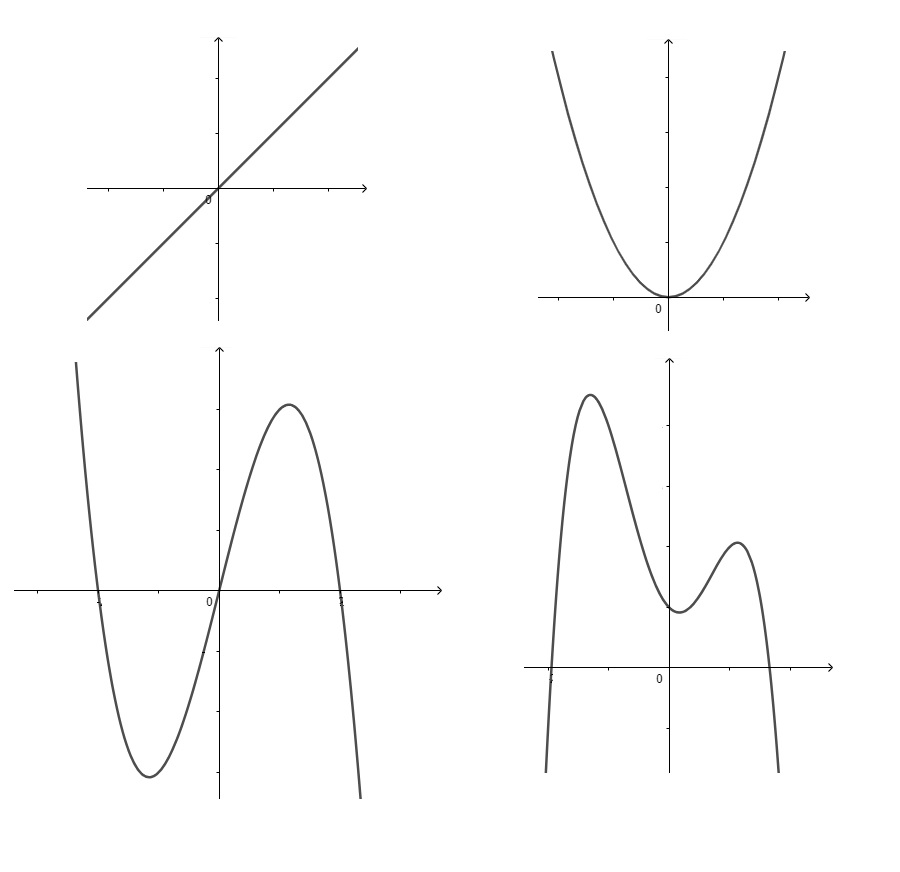
\includegraphics[width=5.8cm]{figures/4graf.jpg}
\end{center}
\end{exemplo}

\end{frame}

%------------------------------------------------------------------------------------------------------------
\begin{frame}
\frametitle{Gráficos de Funções Polinomiais} %\framesubtitle{Exemplos}
 Sejam $p$ e $q$ dois polinômios.

\begin{itemize}
	\item Se o grau de $p$ é maior do
	que o grau de $q$, então para todo $x$ com valor absoluto
	suficientemente grande, tem-se $\modu {p(x)} > \modu{q(x)}$;
	\pause
	\item Sejam $x_1, x_2 \in \R$. Se $p(x_1) < 0$ e $p(x_2)>0$,
	então,
	$p$ deve possuir uma raiz entre $x_1$ e $x_2$.
\end{itemize}

\end{frame}

%------------------------------------------------------------------------------------------------------------
\begin{frame}
\frametitle{Gráficos de Funções Polinomiais} %\framesubtitle{Exemplos}
\begin{exemplo}\label{exemfig}
Considere os polinômios $p(x) = x^7 $ e $q(x)=x^3$. Quando $0< \modu
x < 1$, temos que $\modu {p(x)} < \modu{q(x)}$. Porém, quando $
\modu x > 1$, temos que $\modu {p(x)} > \modu{q(x)}$. Além disso, em
ambos os casos, $p(-1) = q(-1) = -1 <0$ e $p(1) = q(1) = 1 >0$.
Assim, os polinômios possuem, cada um, ao menos uma raiz no
intervalo $(-1, 1)$ -- a saber, $x=0$.

\end{exemplo}

\end{frame}

%------------------------------------------------------------------------------------------------------------
\begin{frame}
\frametitle{Gráficos de Funções Polinomiais} %\framesubtitle{Exemplos}
\begin{block}{Exemplo \ref{exemfig} (Continuação)}


\begin{center}
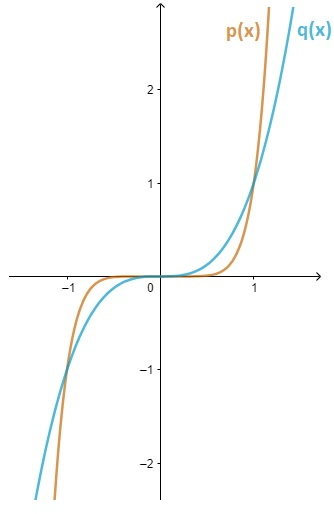
\includegraphics[width=4.3cm]{figures/2graf.jpg}
\end{center}


\end{block}

\end{frame}

%------------------------------------------------------------------------------------------------------------
\section{Atividade Online}
\begin{frame}
\frametitle{Atividade Online} %\framesubtitle{Exemplos}

\href{https://pt.khanacademy.org/math/algebra2/polynomial-functions/zeros-of-polynomials-and-their-graphs/e/using-zeros-to-graph-polynomials}
{{\tt Atividade 09 - Zeros de Polinômios e seus Gráficos}}


Veja o desempenho na Missão Álgebra II.


\end{frame}


%------------------------------------------------------------------------------------------------------------

\section{Exercícios}
\begin{frame}
\frametitle{Exercícios} %\framesubtitle{Exemplos}
\Ex{A escala $N$ de temperaturas foi feita com base nas temperaturas
máxima e mínima em Nova Iguaçu. A correspondência com a escala
Celsius é a seguinte:
\begin{center}
\begin{tabular}{|r|r|}
	\hline
	% after \\: \hline or \cline{col1-col2} \cline{col3-col4} ...
	ºN & ºC \\ \hline
	0 & 18 \\ \hline
	100 & 43 \\
	\hline
\end{tabular}
\end{center}
Modele o problema com funções afim que transformem a temperatura em
ºN em ºC e vice-versa. Qual a relação entre essas duas funções? Em
que temperatura ferve a água na escala $N$?}

\Ex{Mostre que uma função afim $f: \R \to \R$ fica inteiramente
determinada quando conhecemos $f(x_1)$ e $f(x_2)$ para $x_1 \neq
x_2$.}

%\Ex{Prove que toda reta não vertical $r$ (as não-paralelas ao eixo
%$y$) é o gráfico de uma função afim.}
\end{frame}


%------------------------------------------------------------------------------------------------------------
\begin{frame}
\frametitle{Exercícios} %\framesubtitle{Exemplos}

\Ex{Pessoas apressadas podem diminuir o tempo gasto em uma escada
rolante subindo alguns degraus da escada no percurso. Para uma certa
escada, observa-se que uma pessoa gasta 30 seg na escada quando
sobre 5 degraus e 20 seg quando sobe 10 degraus. Quantos são os
degraus da escada e qual o tempo gasto no percurso?}



\Ex{Dada as PA's $\paren{a_1, a_2, \dots, a_n, \dots}$, de razão não
nula, e $\paren{b_1, b_2, \dots, b_n, \dots}$, mostre que existe
uma, e somente uma, função afim $f: \R \to \R$ tal que $f(a_1) =
b_1$, $f(a_2) = b_2$, \dots , $f(a_n) = b_n$, \dots}
\end{frame}

%------------------------------------------------------------------------------------------------------------
\begin{frame}
\frametitle{Exercícios} %\framesubtitle{Exemplos}

\Ex{Os termos $a_1, a_2, \dots, a_n, \dots$ de uma PA são os valores
$f(1), f(2), \dots, f(n), \dots$ de uma função afim, tal que $f(n)
>0$ para todo $n \in \N^\ast$.
\begin{enumerate}[(a)]
	\item Mostre que cada $a_i$ é igual à área de um trapézio
	delimitado pelo gráfico de $f$, pelo eixo $x$ e pelas retas
	verticais de equações $x=i - \frac 1 2 $ e $x = i + \frac 1 2$.
	\begin{center}
\includegraphics[width=4.5cm]{figures/paralelogramo.jpg}
\end{center}
	\item Mostre, por indução, que a soma $S_n = a_1+a_2+ \dots + a_n$ é igual à
	área do trapézio delimitado pelo gráfico de $f$, pelo eixo $x$ e
	pelas retas verticais $x= \frac 1 2$ e $x = n + \frac 1 2 $.
	\item Conclua, a partir da área do trapézio, que $S_n = \frac{a_1+a_n} 2 n$.
\end{enumerate}
}



\end{frame}


%------------------------------------------------------------------------------------------------------------



\begin{frame}
\frametitle{Exercícios} %\framesubtitle{Exemplos}

\Ex{Para cada uma das funções quadráticas abaixo, escreva-a na forma
$f(x)=a(x-m)^2+k$. A seguir, calcule suas raízes (se existirem), o
eixo de simetria de seu gráfico e seu valor mínimo e máximo.
\begin{enumerate}[(a)]
	\item $f(x) = x^2 -8x +23$;
	\item $f(x) = 8x - 2x^2$.
\end{enumerate}
}

\Ex{Encontre os valores mínimo e máximo assumidos pela função $f(x)
= x^2 -4x +3$ em cada um dos intervalos abaixo:
\begin{enumerate}[(a)]
	\item $\colc{1, 4}$;
	\item $\colc{6, 10}$.
\end{enumerate}
\emph{Dica: } Esboce o gráfico de $f(x)$ nos intervalos indicados
para visualizar melhor os valores mínimo e máximo assumidos pela
função.}

\Ex{Os alunos de uma turma fizeram uma coleta para juntar 405 reais,
custo de uma excursão. Todos contribuíram igualmente. Na última
hora, dois alunos desistiram. Com isso, a parte de cada um sofreu um
aumento de um real e vinte centavos. Quantos alunos tem a turma? }

\end{frame}



%------------------------------------------------------------------------------------------------------------

\begin{frame}
\frametitle{Exercícios} %\framesubtitle{Exemplos}

\Ex{Determine o polinômio $p(x)$ de menor grau possível tal que
$p(1) = 2$, $p(2)=1$, $p(3) = 4$ e $p(4) = 3$. }

\Ex{Mostre que, se $n$ é um número par, então o polinômio $p(x) =
x^n + x^{n-1} + \dots + x+1$ não possui raiz real.
\\
\emph{Dica: } Note que, para $x \neq 1$, $p(x) =
\frac{x^{n+1}-1}{x-1}$. Proceda supondo, por contradição, que existe
$a \neq 1$ raiz de $p(x)$.}

\end{frame}

\section{Bibliografia}

\frame{
	\frametitle{Bibliografia}

	\begin{thebibliography}{99}
		\bibitem {label1}
		LIMA, Elon L; CARVALHO, Paulo César P; Wagner, Eduardo; MORGADO,
		Augusto C.
		\newblock \emph{A Matemática do Ensino Médio. Vol. 1}.
		\newblock 9. ed. Rio de Janeiro: SBM, 2006.

		\bibitem {label2}
		IEZZI, Gelson; et al.
		\newblock \emph{Fundamentos de Matemática Elementar. Vol. 1 - Conjuntos e Funções}.
		\newblock São Paulo: Editora Atual.
	\end{thebibliography}
}

\end{document}
